\documentclass[../delivery_hospital_report.tex]{subfiles}
\graphicspath{ {images/}{../images/} } 

\begin{document}
\chapter{Modulos Embarcados}

\begin{figure}[h]
\centering
    \caption{Módulos Embarcados - Robô Hospitalar (V2)}
    \centering % para centralizarmos a figura
    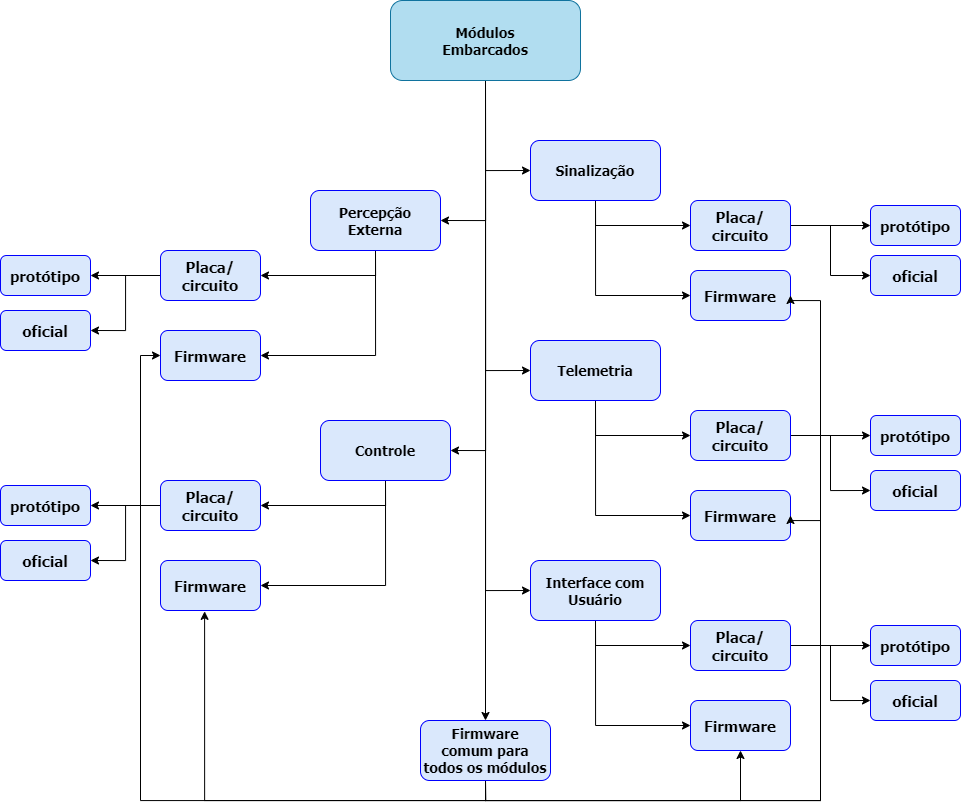
\includegraphics[width=16cm]{modulos_embarcados.png}
    \caption*{Fonte: Elaborada pelo autor}
    \label{figura:1° Versão Robô Hospitalar}
\end{figure}


###
comentar:
modulos disponibilzados no github
-padronização:
    prototipo:
        - micro
        - tamanho de placa
        - local dos componentes
        - encapsulamento
    oficial
        - micro
         - tamanho de placa
        - local dos componentes
        - encapsulamento

%================================ FIRMWARE PARA TODOS ========================
\section{Firmware comum para todos os módulos}

%================================ CONTROLE ========================

\subfile{modulos/controle}

%================================ PERCEPÇÂO EXTERNA ========================

\subfile{modulos/percepcao}

%================================ SINALIZAÇÂO ========================

\subfile{modulos/sinalizacao}

%================================ TELEMETRIA ========================

\subfile{modulos/telemetria}

%================================ INTERFACE COM USUARIO ========================

\subfile{modulos/interface}


\end{document}